\documentclass[11pt,letterpaper]{article}
\usepackage[top=0.85in,left=2.00in,footskip=0.75in]{geometry}
\usepackage[titletoc,page]{appendix}
% Use adjustwidth environment to exceed column width (see example table in text)
\usepackage{changepage}
\usepackage[english]{babel}
\usepackage{booktabs}
\usepackage{siunitx}%Questo serve a caricare il pacchetto delle unità di misura del sistema internazionale%
\usepackage[utf8]{inputenc}
\usepackage{graphicx} 
\usepackage{url}
\usepackage{amsmath}
\usepackage{amssymb}
\usepackage{listings}


\usepackage{keyval}
\usepackage{xcolor}
\usepackage{caption}
\usepackage{tikz}
\usepackage{circuitikz}
\usepackage{authblk}
%\usepackage{hyperref}


\usepackage[lofdepth,lotdepth]{subfig}
% Remove comment for double spacing
%\usepackage{setspace} 
%\doublespacing
% Text layout
%\raggedright
\setlength{\parindent}{0.5cm}
\textwidth 5.25in 
\textheight 8.75in

\usepackage[aboveskip=1pt,labelfont=bf,labelsep=period,justification=raggedright,singlelinecheck=off]{caption}

% Use the PLoS provided BiBTeX style
\bibliographystyle{plos2009}

% Remove brackets from numbering in List of References
\makeatletter
\renewcommand{\@biblabel}[1]{\quad#1.}
\makeatother


\begin{document}
\vspace*{0.30in}

\begin{flushleft}
{\Large
\textbf\newline{\textbf{Optical tweezers - Kramers escape rate}}
}
\newline
% Insert Author names, affiliations and corresponding author email.
\\
Lorenzo Maria Perrone\textsuperscript{1, *}
%Name2 Surname\textsuperscript{2,\textpilcrow},
%Name3 Surname\textsuperscript{2,\textcurrency a},
%Name4 Surname\textsuperscript{2,\ddag},
%Name5 Surname\textsuperscript{2,\ddag},
%Name6 Surname\textsuperscript{2,\Yinyang},
%Name7 Surname\textsuperscript{3,*,\Yinyang}
\\
\bf{1} Department of Physics, EPFL
\\
%\bf{2} Affiliation Dept/Program/Center, Institution Name, City, State, Country
%\\
%\bf{3} Affiliation Dept/Program/Center, Institution Name, City, State, Country
%\\

% Insert additional author notes using the symbols described below. Insert symbol callouts after author names as necessary.
% 
% Remove or comment out the author notes below if they aren't used.
%
% Primary Equal Contribution Note
%\Yinyang These authors contributed equally to this work.

% Additional Equal Contribution Note
%\ddag These authors also contributed equally to this work.

% Current address notes
%\textcurrency a Insert current address of first author with an address update
% \textcurrency b Insert current address of second author with an address update
% \textcurrency c Insert current address of third author with an address update

% Deceased author note
%\dag Deceased

% Group/Consortium Author Note
%\textpilcrow Insert Collaborative Author line here

* E-mail: lorenzo.perrone@epfl.ch
\end{flushleft}

\section{Axial potential V(z)}
\begin{figure}[!h]
\centering
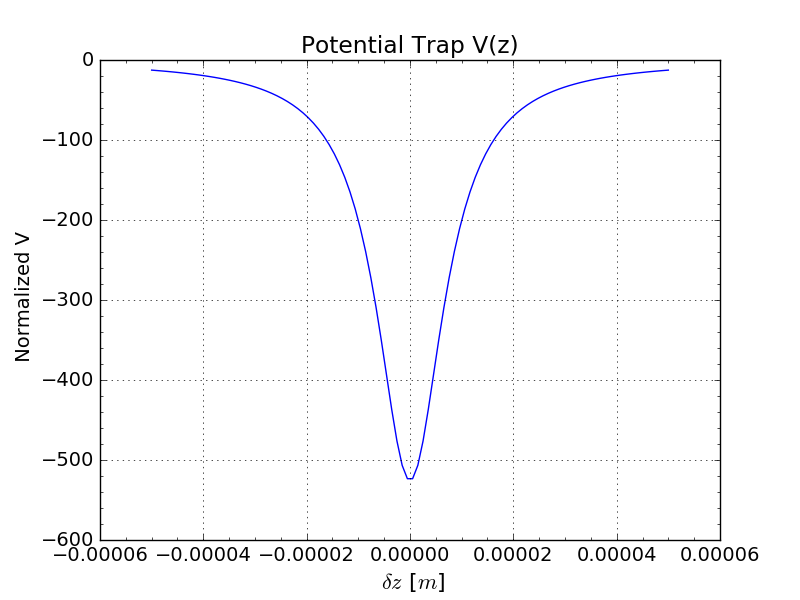
\includegraphics[width=0.9\linewidth]{./V(z)}
\caption{Potential profile for longitudinal force.}
\label{fig:potential}
\end{figure}

\end{document}